%iffalse
\let\negmedspace\undefined
\let\negthickspace\undefined
\documentclass[journal,12pt,onecolumn]{IEEEtran}
\usepackage{cite}
\usepackage{amsmath,amssymb,amsfonts,amsthm}
\usepackage{algorithmic}
\usepackage{graphicx}
\usepackage{textcomp}
\usepackage{xcolor}
\usepackage{txfonts}
\usepackage{listings}
\usepackage{enumitem}
\usepackage{mathtools}
\usepackage{gensymb}
\usepackage{comment}
\usepackage[breaklinks=true]{hyperref}
\usepackage{tkz-euclide} 
\usepackage{listings}
\usepackage{gvv}       
\usepackage{circuitikz}
%\def\inputGnumericTable{}                                 
\usepackage[latin1]{inputenc}                                
\usepackage{color}                                            
\usepackage{array}                                            
\usepackage{longtable}                                       
\usepackage{calc}                                             
\usepackage{multirow}                                         
\usepackage{hhline}                                           
\usepackage{ifthen}                                           
\usepackage{lscape}
\usepackage{tabularx}
\usepackage{array}
\usepackage{float}


\newtheorem{theorem}{Theorem}[section]
\newtheorem{problem}{Problem}
\newtheorem{proposition}{Proposition}[section]
\newtheorem{lemma}{Lemma}[section]
\newtheorem{corollary}[theorem]{Corollary}
\newtheorem{example}{Example}[section]
\newtheorem{definition}[problem]{Definition}
\newcommand{\BEQA}{\begin{eqnarray}}
\newcommand{\EEQA}{\end{eqnarray}}
\newcommand{\define}{\stackrel{\triangle}{=}}
\theoremstyle{remark}
\newtheorem{rem}{Remark}

% Marks the beginning of the document
\begin{document}
\bibliographystyle{IEEEtran}
\vspace{3cm}

\title{2014-EE-27-39}
\author{AI24BTECH11011 - Himani Gourishetty}
\maketitle
\bigskip

\renewcommand{\thefigure}{\theenumi}
\renewcommand{\thetable}{\theenumi}
\begin{enumerate}
 \item A fair coin is tossed n times. The probability that the difference between the number of heads and tails is $\brak{n-3}$ is
 \begin{enumerate}
     \item $2^{-n}$
\item 0
\item $^{n}C_{n-3}2^{-n}$
\item $2^{-n+3}$
 \end{enumerate}
 \item The line integral of function \textbf{F} = yz\textbf{i}, in the counterclockwise direction, along the circle $x^{2} + y^{2}$= 1 at $z= 1$ is
\begin{enumerate}
    \item -2$\pi$
    \item -$\pi$
    \item $\pi$
    \item 2$\pi$
\end{enumerate}
\item An incandescent lamp is marked 40W, 240V. If resistance at room temperature $\brak{26^\degree C}$ is 120$\ohm$, and temperature coefficient of resistance is $4.5\times10^{-3}/\degree C$, then is 'ON' state filament temperature in $\degree C$ is approximately $\makebox[3cm][l]{\underline{\hspace{1cm}}}$

\item In the figure, the value of resistor R is $\brak{25 + \frac{I}{2}}$ ohms, where I is the current in amperes. The current I is $\makebox[3cm][l]{\underline{\hspace{1cm}}}$ 
\begin{figure}[!ht]
\centering
\resizebox{0.4\textwidth}{!}{
	
\begin{circuitikz}
\tikzstyle{every node}=[font=\normalsize]
\draw [->, >=Stealth, dashed] (2.5,8.75) -- (2.5,15.75);
\draw [->, >=Stealth, dashed] (2.5,9) -- (20,9);
\draw [dashed] (2.5,10.5) -- (19.75,10.5);
\draw [->, >=Stealth] (3.5,10.5) -- (3.5,14.5);
\draw [short] (3.5,10.5) -- (5,10.5);
\draw [short] (5,10.5) -- (5,9);
\draw [short] (5,9) -- (7.5,9);
\draw [->, >=Stealth] (7.5,9) -- (7.5,14.5);
\draw [->, >=Stealth] (9.75,9) -- (9.75,14.5);
\draw [short] (9.75,9) -- (11,9);
\draw [short] (11,9) -- (11,10.5);
\draw [short] (11,10.5) -- (12.5,10.5);
\draw [short] (12.5,10.5) -- (12.5,9);
\draw [short] (12.5,9) -- (13.75,9);
\draw [->, >=Stealth] (14,9) -- (14,14.5);
\draw [->, >=Stealth] (15.5,10.5) -- (15.5,14.5);
\draw [short] (15.5,10.5) -- (16,10.5);
\draw [short] (16,10.5) -- (16,9);
\draw [short] (16,9) -- (18.5,9);
\draw [short] (18.5,9) -- (18.5,10.5);
\draw [short] (18.5,10.5) -- (19,10.5);
\draw [->, >=Stealth] (19,10.5) -- (19,14.5);
\node [font=\normalsize] at (2,10.25) {V};
\node [font=\scriptsize] at (2.25,10.25) {0};
\node [font=\normalsize] at (5.5,13.5) {(i)};
\node [font=\normalsize] at (12,13.5) {(ii)};
\node [font=\normalsize] at (17,13.5) {(iii)};
\node [font=\normalsize] at (4.25,11) {L/3};
\node [font=\normalsize] at (10.25,11) {L/3};
\node [font=\normalsize] at (11.75,11) {L/3};
\node [font=\normalsize] at (15.75,11) {L/6};
\node [font=\normalsize] at (17.25,9.5) {2L/3};
\draw [<->, >=Stealth] (3.75,10.75) -- (4.75,10.75);
\draw [<->, >=Stealth] (9.75,10.75) -- (10.75,10.75);
\draw [<->, >=Stealth] (11,10.75) -- (12.5,10.75);
\draw [<->, >=Stealth] (15.5,10.75) -- (16,10.75);
\draw [<->, >=Stealth] (16.25,9.25) -- (18.25,9.25);
\node [font=\normalsize] at (2.25,9) {0};
\end{circuitikz}

}%
\end{figure}
\item In an unbalanced three phase system, phase current $I_{a} = 1{\langle}\brak{-90\degree}pu$ negative sequence current $I_{b2} = 4{\langle}\brak{-150{\degree}}pu$, zero sequence current $I_{c0} = 3\langle{-90\degree}pu$. The magnitude of phase current $I_b$ in pu is
\begin{enumerate}
    \item 1.00
    \item 7.81
    \item 11.53
    \item 13.00
\end{enumerate}
\item The following four vector fields are given in Cartesian co-ordinate system. The vector field which does not satisfy the property of magnetic flux density is
\begin{enumerate}
    \item $y^{2}a_{x} + z^{2}a_{y} + x^^2a_{z}$
    \item $z^{2}a_{x} + x^{2}a_{y} + y^{2}a_{z}$
    \item $x^{2}a_{x} + y^{2}a_{y} + z^{2}a_{Z}$
    \item $y^{2}z^{2}a_{x} + x^{2}z^{2}a_{y} + x^{2}y^{2}a_{Z}$
\end{enumerate}
\item The function shown in the figure can be represented as\\
\begin{figure}[h!]
\centering
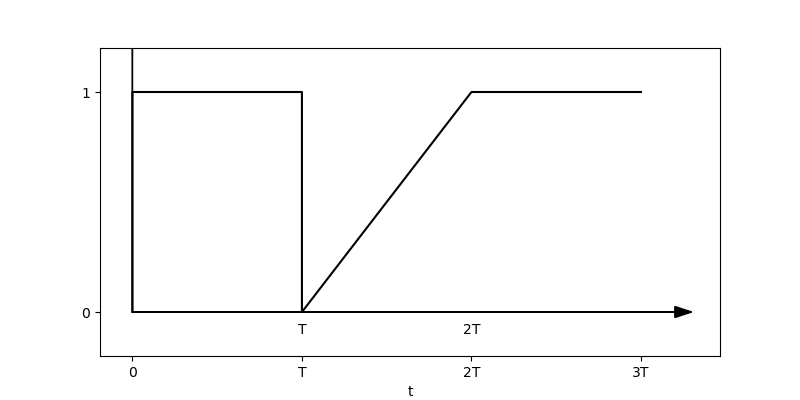
\includegraphics[width=0.4\linewidth]{figs/graph.png}
\label{fig:11011}
\end{figure}
\begin{enumerate}
    \item $u\brak{t} - u\brak{t-T} + \frac{\brak{t-T}}{T}u\brak{t-T} - \frac{\brak{t-2T}}{T}u\brak{t-2T}$
    \item $u\brak{t} + \frac{t}{T}u\brak{t-T} - \frac{t}{T}u\brak{t-2T}$
    \item $u\brak{t} - u\brak{t-T} + \frac{\brak{t-T}}{T}u\brak{t}- \frac{\brak{t-2T}}{T}u\brak{t}$
    \item $u\brak{t} + \frac{\brak{t-T}}{T}u\brak{t-T} - 2\frac{\brakt-2T}}{T}u\brak{t-2T}$
\end{enumerate}
\item Let $ X\brak{z} = \frac{1}{1 - z^{-3}}$ be the Z-transform of a casual signal x[n]. Then, the values of x[2] and x[3] are
\begin{enumerate}
    \item 0 and 0
    \item 0 and 1
    \item 1 and 0
    \item 1 and 1
\end{enumerate}
\item Let f$\brak{t}$ be a continuous time signal and let F$\brak{\omega}$ be its Fourier Transform $$F\brak{\omega}=\int_{-\infty}^{\infty} f\brak{t}e^{-j\omega t} dt$$
Define g$\brak{t}$ by $$g\brak{t} = \int_{-\infty}^{\infty} F\brak{u}e^{-jut} du$$
What is the relationship between f$\brak{t}$
and g$\brak{t}$ ?
\begin{enumerate}
    \item g$\brak{t}$ would always be proportional to f$\brak{t}$.
    \item g$\brak{t}$ would be proportional to f$\brak{t}$ if f$\brak{t}$ is an even function.
    \item g$\brak{t}$ would be proportional to f$\brak{t}$ only if f$\brak{t}$ is a sinusoidal function.
    \item g$\brak{t}$ would never be proportional to f$\brak{t}$
\end{enumerate}
\item The core loss of a single phase, 230/115V, 50Hz power transformer is measured from 230V side by feeding the primary $\brak{230 V side}$ from a variable voltage frequency source while keeping th secondary open circuited. The core loss is measured to be 1050 W for 230 V, 50 Hz input. The core loss is again measured to be 500 W for 138 V, 30 Hz input. The hysteresis and eddy current losses of the transformer for 230 V, 50 Hz input are respectively,
\begin{enumerate}
    \item 508 W and 542 W
    \item 468 W and 582 W
    \item 498 W and 552 W
    \item 488 W and 562 W
\end{enumerate}
\item A 15 kW, 230 V de shunt motor has armature circuit resistance of $0.4\ohm$ and field circuit resistance of $230\ohm$. At no load and rated voltage, the motor runs at 1400 rpm and the line current drawn by the motor is 5 A. At full load, the motor draws a line current of 70 A. Neglect the armature reaction. The full load speed of the motor in rpm is $\makebox[3cm][l]{\underline{\hspace{1cm}}}$.

\item A 3 phase, 50 Hz, six pole induction motor has a rotor resistance of $0.1\ohm$ and reactance of $0.92\ohm$. Neglect the voltage drop in stator and assume that the rotor resistance is constant. Give that the full load slip is $3\%$, the ratio maximum torque to full load torque is
\begin{enumerate}
    \item 1.567
    \item 1.712
    \item 1.948
    \item 2.134
\end{enumerate}
\item A three phase synchronous generator is to be connected to the infinite bus. The lamps are connected as shown if the figure for the synchronization. The phase sequence of bus voltage is R-Y-B and that of incoming generator voltage is R'-Y'-B'.
\begin{figure}[!ht]
\centering
\resizebox{0.4\textwidth}{!}{
	\begin{circuitikz}
\tikzstyle{every node}=[font=\normalsize]
\draw [short] (1.5,10.5) -- (1.5,6.5);
\draw [short] (1.5,6.5) -- (5,6.5);
\draw [short] (8,10.75) -- (5.5,10.75);
\draw [short] (5.5,10.75) -- (5.5,6.5);
\draw [short] (5.5,6.5) -- (8.25,6.5);
\draw [short] (10.25,10.75) -- (10.25,6.5);
\draw [short] (8.5,10.75) -- (11.75,10.75);
\draw [short] (14,10.75) -- (14,6.5);
\draw [short] (12,8.5) -- (15.75,8.5);
\draw [line width=1.2pt, ->, >=Stealth] (1.5,8.75) -- (1.5,6.75);
\draw [line width=1.2pt, ->, >=Stealth] (5.5,8.75) -- (5.5,6.75);
\draw [line width=1.2pt, ->, >=Stealth] (10.25,10.75) -- (10.25,8.75);
\draw [line width=1.2pt, ->, >=Stealth] (14,8.5) -- (14,7);
\node at (1.5,6.5) [circ] {};
\node at (5.5,8.75) [circ] {};
\node at (10.25,10.75) [circ] {};
\node at (14,8.5) [circ] {};
\node [font=\normalsize] at (1.25,6.5) {P};
\node [font=\normalsize] at (2,8) {F};
\node [font=\normalsize] at (5.25,8.75) {P};
\node [font=\normalsize] at (5.75,6.75) {F};
\node [font=\normalsize] at (10,10.5) {P};
\node [font=\normalsize] at (10.5,8.75) {F};
\node [font=\normalsize] at (13.75,8.75) {P};
\node [font=\normalsize] at (14.25,7) {F};
\node [font=\normalsize] at (1.5,11) {Case(i)};
\node [font=\normalsize] at (5.75,11.25) {case(ii)};
\node [font=\normalsize] at (9,11.25) {case(iii)};
\node [font=\normalsize] at (12.75,11.25) {case(iv)};
\end{circuitikz}

}%
\end{figure}
It was found that the lamps are becoming dark in the sequence $L_{a}-L_{b}-L_{c}$. It means that the phase sequence of incoming generator is
\begin{enumerate}
    \item opposite to infinite bus and its frequency is more than infinite bus
    \item opposite to infinite bus but its frequency is less than infinite bus
    \item same as infinite bus and its frequency is more than infinite bus
    \item same as infinite bus and its frequency is less than infinite bus
\end{enumerate}
\end{enumerate}


\end{document}
